\documentclass{article}
\usepackage{graphicx}
\usepackage{amsmath}
\PassOptionsToPackage{svgnames}{xcolor}
\usepackage{tcolorbox}
\usepackage{xcolor}
\usepackage{lipsum}
\usepackage{verbatim}
\tcbuselibrary{skins,breakable}
\usetikzlibrary{shadings,shadows}
\usepackage{float}
\usepackage{hyperref}
\usepackage[a4paper]{geometry}
\usepackage{listings}
\usepackage{titlesec}
\usepackage{amssymb}
\usepackage[T1]{fontenc}
\usepackage{multirow} % for Tables
\usepackage{fancyvrb} % for "\Verb" macro
\VerbatimFootnotes % enable use of \Verb in footnotes
\usepackage{listings}
\lstset{basicstyle=\ttfamily,
  showstringspaces=false,
  commentstyle=\color{green},
  keywordstyle=\color{blue}
}

\setcounter{secnumdepth}{4}
\titleformat{\paragraph}
{\normalfont\normalsize\bfseries}{\theparagraph}{1em}{}
\titlespacing*{\paragraph}
{0pt}{3.25ex plus 1ex minus .2ex}{1.5ex plus .2ex}

\title{\textbf{Apunts de Probabilitat}}
\author{Alejandro Campos}
\date{August, 2023}

\setlength{\parindent}{0ex}
\setlength{\parskip}{6pt}
\geometry{top=2.5cm, bottom=3cm,left=3cm, right=3cm}
\hypersetup{
    colorlinks=true,
    linkcolor=black,
    filecolor=magenta,      
    urlcolor=blue,
}

\definecolor{codegreen}{rgb}{0,0.6,0}
\definecolor{codegray}{rgb}{0.5,0.5,0.5}
\definecolor{codepurple}{rgb}{0.58,0,0.82}
\definecolor{backcolour}{rgb}{0.95,0.95,0.92}

\newenvironment{blocktemplate}[1]{%
    \tcolorbox[beamer,%
    noparskip,breakable,
    colframe=Blue,%
    colbacklower=LimeGreen!75!LightGreen,%
    title=#1]}%
    {\endtcolorbox}

\newenvironment{blocktemplateI}[1]{%
    \tcolorbox[beamer,%
    noparskip,breakable,
    colframe=Violet,%
    colbacklower=Black,%
    title=#1]}%
    {\endtcolorbox}

\newenvironment{blocktemplateII}[1]{%
    \tcolorbox[beamer,%
    noparskip,breakable,
    colframe=Green,%
    colbacklower=LimeGreen!75!LightGreen,%
    title=#1]}%
    {\endtcolorbox}

\newenvironment{blocktemplateIII}[1]{%
    \tcolorbox[beamer,%
    noparskip,breakable,
    ,colframe=Red,%
    colbacklower=LimeGreen!75!LightGreen,%
    title=#1]}%
    {\endtcolorbox}

\newtcolorbox{mybasecolorbox}[1][]{%
  colback=gray!25, colframe=gray!25,
  coltitle=black,
  width=(\linewidth-20pt)}

\newenvironment{codetemplate}[1][]{%
  \mybasecolorbox[#1]
  \itshape
}{%
  \endmybasecolorbox
}

\begin{document}
\maketitle
\newpage
\tableofcontents

%====================================================================================================
\newpage

\section{Introducció a la Probabilitat}

\subsection{Significat de la Probabilitat}

La probabilitat és una mesura de la certesa de que un determinat esdeveniment es produeixi. El seu valor és sempre un número entre 0 i 1, on un event imposible correspon a 0 i un de segur correspon a 1.

Distingim dos tipus de processos:
\begin{itemize}
    \item \textbf{Deterministes:} Les condicions del sistema determinen completament el seu comportament. Si repetim l’experiment en les mateixes condicions sempre obtenim el mateix resultat. Per exemple, mesurar amb quina velocitat arriba a terra una pedra deixada caure des de 1m d’alçada.
    \item \textbf{Aleatòris:} Fixades les condicions, el sistema admet més d’un comportament possible. Al repetir l’experiment anem obtenint resultats diferents. Per exemple, tirar un dau.
\end{itemize}

La probabilitat també es pot interpetar freqüencialment. Siguin:
\begin{itemize}
    \item $\mathcal{E}:$ un experiment aleatori
    \item $A:$ un resultat de l'experiment
    \item $N:$ nombre de vegades que es realitza l'experiment
    \item $N_A:$ nombre de vegades que succeeix $A$
\end{itemize}

Definim la freqüencia relativa de $A$ com $f_A = \dfrac{N_A}{N}$.\\

Llavors esperem que: $\displaystyle \lim_{N\to\infty} f_A = \displaystyle \lim_{N\to\infty} \dfrac{N_A}{N} = P(A)$

L’expressió diu que si fem moltes vegades l’experiment, $f_A$ hauria de prendre valors molt propers a $P(A)$. Així, una forma empírica d'estimar la probabilitat d'un determinat esdeveniment consisteix en calcular la freqüencia amb la que succeeix aquest esdeveniment mitjançant la repetició de l'experiment aleatori, sota condicions suficientement estables. 

\subsection{Conceptes Bàsics}
\subsubsection{Experiment Aleatori}
$\mathcal{E}$ s'anomena experiment aleatori: experiment que es pot repetir tantes vegades com es vulgui sempre en les mateixes condicions.

\subsubsection{Espai Mostral}
$\Omega$ s'anomena espai mostral i es el conjunt dels possibles resultats d'un experiment aleatori $\mathcal{E}$.

\underline{Exemple 1}
\begin{itemize}
    \item $\mathcal{E}$ = “Tirar una moneda dues vegades”
    \item $\Omega$ = \{oo, o+, +o, ++\}
\end{itemize}

\underline{Exemple 2}
\begin{itemize}
    \item $\mathcal{E}$ = “Tirar un dau"
    \item $\Omega$ = \{1, 2, 3, 4, 5, 6\}
\end{itemize}

\subsubsection{Esdeveniment Aleatori}
Donat un experiment $\mathcal{E}$, un esdeveniment aleatori és una proposició lògica A tal que a l’efectuar una
prova de $\mathcal{E}$ podem determinar la seva veritat o falsedat. Per tant A es sempre un subconjunt de $\Omega$, $A\in\Omega$. Per abús del llenguatge utilitzem el mateix nom per l'esdeveniment aleatori i el subconjunt que el forma. El complementari d'A, $\Omega$ - A, l'anomenem $\overline{A}$.

S'anomena conjunt vuit $\emptyset$, al esdeveniment imposible.

\underline{Exemple 1}
\begin{itemize}
    \item $\mathcal{E}$ = “Tirar un dau”
    \item $\Omega$ = \{1, 2, 3, 4, 5, 6\}
    \item A = "Que surti parell" = \{2, 4, 6\}
    \item $\overline{A}$ = "Que no surti parell" = \{1, 3, 5\}
    \item B = "Que surti multiple de 3" = \{3, 6\}
    \item $\overline{B}$ = "Que no surti multiple de 3" = \{1, 2, 4, 6\} 
    \item $\emptyset$ = "Treure multiple de 7"
\end{itemize}

\subsubsection{Propietats}

Donats els esdeveniments aleatoris A i B, sempre es compleix:
\begin{enumerate}
    \item $P(\emptyset) = 0$
    \item $P(\overline{A}) = 1 - P(A)$
    \item $P(A) \leq 1$
    \item $P(A \cup B) = P(A) + P(B) - P(A \cap B)$
    \item $P(A \cap B) = P(B \cap A) = P(A) \cdot P(B \mid A) = P(B) \cdot P(A \mid B)$ 
    \item $P(A \cup B \cup C) = P(A) + P(B) + P(C) - P(A \cap B) - P(A \cap C) - P (B \cap C) - P(A \cap B \cap C)$
\end{enumerate}

\begin{figure}[H]
    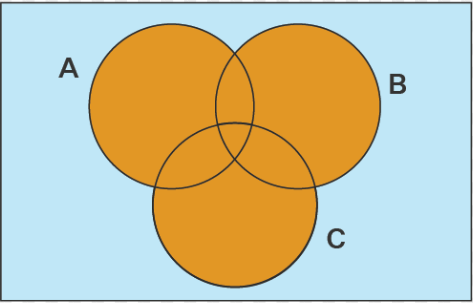
\includegraphics[scale=0.35]{pictures/image3.png}
    \centering
\end{figure}


\subsubsection{Factorial}
Donat $m$ natural, anomenarem factorial de $m$ el producte dels $m$ primers naturals, és a dir, $m! = m \cdot (m-1) \cdot \ldots \cdot 1$

Per notació considerarem $0! = 1$. Observeu que $1! = 1$ i que $m! = m \cdot (m - 1)!$.

\subsection{Combinatòria}
Per poder calcular les probabilitats més senzilles, la primera cosa que necessitem saber es comptar el nombre de resultats possibles d’un experiment, es a dir, els cardinals de conjunts, $|A|$. 

Donal el conjunt $\{A, B, C, D, E, F, G$\}, quantes paraules diferents es poden formar amb aquestes lletres? Abans de respondre, ens hauriem de fer les següents preguntes:

\begin{itemize}
    \item Paraules de quantes lletres?
    \item Es poden repetir les lletres?
    \item Dues paraules amb les mateixes lletres ordenades de manera diferent son la mateixa paraula?
\end{itemize}

Aquestes son les 3 preguntes bàsiques que ens hem de fer a l'hora de decidir com comptar el nombre de resultats possibles d'un experiment.

\subsubsection{La regla del producte}
Suposem que hem d’efectuar $k$ tries successives. Si tenim $m_{1}$ possibilitats en la primera tria, $m_{1}$ possibilitats per a la segona tria, i així successivament, $m_{k}$ possibilitats per a la $k-$èsima tria, aleshores el nombre total d’eleccions possibles és de $m_{1} \cdot m_{2} \cdot m_{2} \cdot \ldots \cdot m_{k}$.

Cal esmentar, que utilitzant aquesta tècnica estem suposant separació entre conjunts. Ho veiem en l'exemple.

\underline{Exemple}

El menú d’un restaurant es compón de 4 primers, 3 segons i 3 postres diferents. Escollint un entrant, un plat i unes postres, quants menús diferents es poden fer?

$4 \cdot 3 \cdot 3 = 36$

Aquesta tècnica està suposant separació de conjunts, doncs no contempla l'opció d'escollir un primer com a segón. En aquest cas l'operació es complicaria.

Aquests càlculs es poden representar mitjançant arbres de decissió, veiem un arbre amb 2 entrants, 2 plats i 3 postres:

$2 \cdot 2 \cdot 3 = 12$

\begin{figure}[H]
    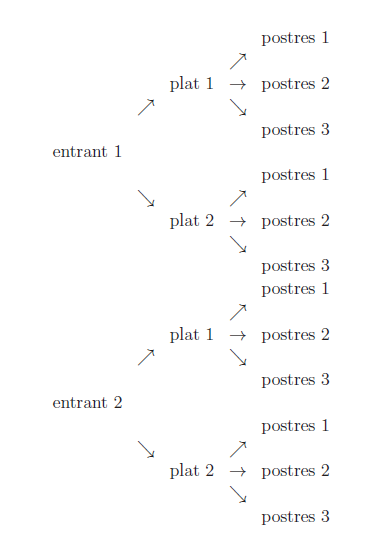
\includegraphics[scale=0.8]{pictures/image2.png}
\end{figure}


\subsubsection{Tècniques per comptar}

\begin{figure}[H]
    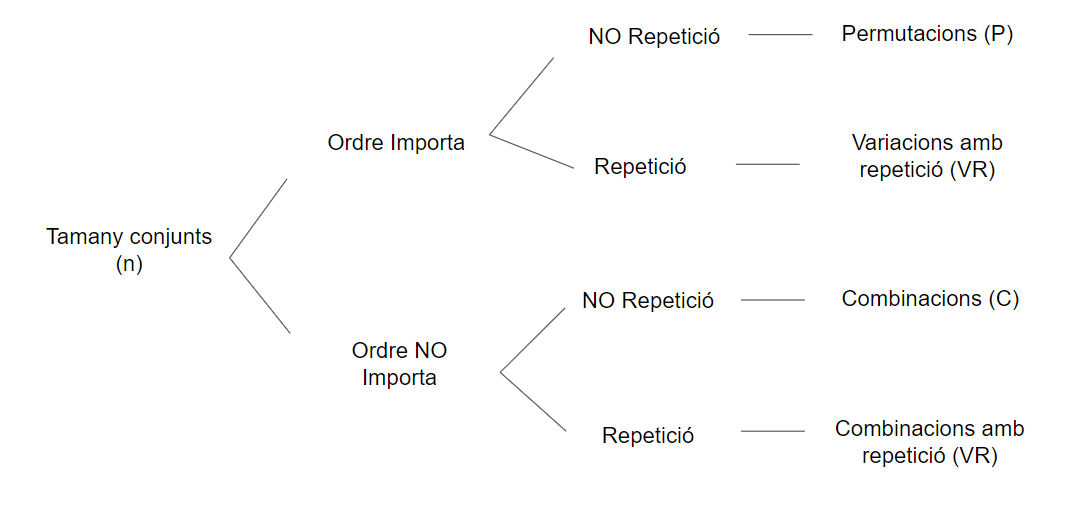
\includegraphics[scale=0.4]{pictures/image1.png}
    \centering
\end{figure}

\paragraph{Variacions i Permutacions}
Total de grups de tamany $k$ que es poden formar amb $m$ elements \textbf{amb ordre i sense repetició}.

\begin{equation*}
V_m^{k} = m \cdot (m-1) \cdot (m-2) \cdot \ldots \cdot (m-k+1) = \dfrac{m!}{(m-k)!}
\end{equation*}

Aquesta formula es deduible seguint \textbf{la regla del producte}. Imaginem una urna amb $m$ boles diferents, quants grups de $k$ elements en podem fer? Seguint la regla del producte, per la primera extracció n'hi ha $m$ elements possibles, per la segona n'hi ha $m-1$, per la terecera n'hi ha $m-2$, i així successivament fins a l'extracció $k$, on tindrem $m-k+1$ elements possibles.

\textbf{Permutacions:} es obvi pero sempre $k \leq m$. En el cas particular $k = m$, parlarem de
permutacions de $m$ elements.

\begin{equation*}
\begin{split}
P_m = m \cdot (m-1) \cdot (m-2) \cdot \ldots \cdot (m-k+1) = m \cdot (m-1) \cdot (m-2) \cdot \ldots \cdot 1 = P_m = m!
\end{split}
\end{equation*}
\begin{align*}
P_m = m!
\end{align*}

\underline{Exemple 1:} fem 3 extraccions d'una urna amb 10 boles diferents sense retornar les boles. Quants grups important l'ordre diferents de boles en podem fer?
\begin{align*}
V_{10}^{3} & = m \cdot (m-1) \cdot (m-2) \cdot \ldots \cdot (m-k+1) = \dfrac{m!}{(m-k)!} \\
           & = 10 \cdot 9 \cdot 8 = \dfrac{10!}{7!} = 720
\end{align*}

\underline{Exemple 2:} Amb les xifres $\{1, 2, 3, 4, 5\}$, quants nombres de 2 xifres diferents podem
escriure sense repetir cap?
\begin{align*}
V_{5}^{2} & = 5 \cdot 4 = 20
\end{align*}

\underline{Exemple 3:} En una lliga de futbol n'hi ha 20 equips diferents. De quantes maneres pot quedar la classificació final?

\begin{align*}
V_{20}^{20} & = P_{20} = 20!
\end{align*}

\underline{Exemple 4:} S'han de repartir 2 premis diferents entre els 100 participants d'un sorteig, de quantes maneres diferents es poden repartir?

\begin{align*}
V_{100}^{2} & = 100 * 99 = 99.000
\end{align*}

\underline{Exemple 5:} Quantes paraules diferents de 5 lletres es poden formar amb el conjunt de lletres $\{A, B, C, D, E, F, G$\} sense repetir-ne cap?
\begin{align*}
V_{7}^{5} & = \dfrac{7!}{5!} = 7 \cdot 6 = 42
\end{align*}

\paragraph{Variacions amb repetició}
Total de grups de tamany $k$ que es poden formar amb $m$ elements \textbf{amb ordre i amb repetició}.

Imaginem l'exemple de la urna amb $m$ boles diferents, però ara retornant les boles, quants grups de $k$ elements en podem fer? Si apliquem la \textbf{regla del producte}:

\begin{equation*}
VR_m^{k} = m^k
\end{equation*}

\underline{Exemple 1:} fem 3 extraccions d'una urna amb 10 boles diferents retornant les boles. Quants grups important l'ordre diferents de boles en podem fer?
\begin{align*}
VR_{10}^{3} & = 10 \cdot 10 \cdot 10 = 10^3
\end{align*}

\underline{Exemple 2:} Amb les xifres $\{1, 2, 3, 4, 5\}$, quants nombres diferents de 4 xifres podem
escriure repetint?
\begin{align*}
VR_{5}^{4} & = 5 * 5 * 5 * 5 = 5^4
\end{align*}

\underline{Exemple 3:} En una travesa de 14 partits, quantes apostes diferents es poden fer? Tenint en comte que pots apostar 1,2 o x (x=empat)
\begin{align*}
VR_{3}^{14} & = 3^{14}
\end{align*}


\paragraph{Combinacions}
Total de grups de tamany $k$ que es poden formar amb $m$ elements \textbf{sense importar l'ordre i sense repetició}.
\begin{equation*}
C_{m}^{k} = \dbinom{m}{k}= \dfrac{m!}{k! \cdot (m-k)!}
\end{equation*}

\underline{Exemple 1:} en una classe de 30 alumnes, quants grups de delegats diferents (3 alumnes) en podem fer?
\begin{align*}
C_{30}^{3} & = \dbinom{30}{3}= \dfrac{30!}{3! \cdot 27!} = \dfrac{30 \cdot 29 \cdot 28}{6} = 4060
\end{align*}

\underline{Exemple 2:} en una barralla de poker (52) cartes, quants grups diferents de 5 cartes es poden fer?
\begin{align*}
C_{52}^{5} & = \dbinom{52}{5}= \dfrac{52!}{5! \cdot 47!} = 2.598.960
\end{align*}

\underline{Exemple 3:} s'han de repartir 2 premis iguals entre 100 persones, de quantes maneres es poden repartir?
\begin{align*}
C_{100}^{2} & = \dbinom{100}{2}= \dfrac{100!}{2! \cdot 98!} = \dfrac{100 \cdot 99}{2} = 4950
\end{align*}

\underline{Exemple 4:} Un cambrer té sucs de taronja, poma, raïm, pinya, meló i pera. Quants sucs diferents pot fer barrejant a parts iguals tres sucs diferents?
\begin{align*}
C_{6}^{3} & = \dbinom{6}{3}= \dfrac{6!}{3! \cdot 3!} = \dfrac{6 \cdot 5 \cdot 4}{3} = 20
\end{align*}

\underline{Exemple 5:} En una loteria de tipus 6/49 tenim un requadre amb 49 nombres dels quals hem de marcar-ne 6, quantes combinacions diferents en podem fer?
\begin{align*}
C_{49}^{6} & = \dbinom{49}{6}= \dfrac{49!}{6! \cdot 43!} = 13.983.816
\end{align*}

\paragraph{Combinacions amb repetició}
Total de grups de tamany $k$ que es poden formar amb $m$ elements \textbf{sense importar l'ordre però amb repetició}.
\begin{equation*}
CR_{m}^{k} = \dbinom{m + k - 1}{k}= \dfrac{m!}{k! \cdot (m-k)!}
\end{equation*}

\underline{Exemple 1:} en una barralla de poker (52) cartes, quants grups diferents de 5 cartes es poden fer tenint en comte que retornem les carta a la baralla?
\begin{align*}
CR_{52}^{5} & = \dbinom{52 + 5 - 1}{2} = \dbinom{56}{5} = 3.819.816
\end{align*}

\underline{Exemple 2:} s'han de repartir 2 premis iguals entre 100 persones, a la mateixa persona li poden tocar els dos premis, de quantes maneres es poden repartir?
\begin{align*}
CR_{100}^{2} & = \dbinom{100 + 2 - 1}{2}= \dbinom{101}{2} =  \dfrac{101 \cdot 100}{2} = 5050
\end{align*}

\underline{Exemple 3:} Un cambrer té sucs de taronja, poma, raïm, pinya, meló i pera. Quants sucs diferents pot fer barrejant a parts iguals tres sucs (pot repetir)?
\begin{align*}
CR_{6}^{3} & = \dbinom{6 + 3 - 1}{3} = \dbinom{8}{3} = 8 \cdot 7 = 56 
\end{align*}

\subsection{Probabilitat Condicionada}

\subsubsection{Esdeveniments Independents}
Diem que dos esdeveniments $A$ i $B$ són independents quan el resultat d'un no afecta al resultat de l'altre. Per exemple, si tirem 2 daus, la primera tirada no afectará en res a la segona. En canvi, si extraiem 2 cartes d'una baralla sense remplaçament ja no son independents, doncs les probabilitats de l'extracció de la segona carta es veuran condicionades per la primera extracció.

Per a 2 esdeveniments independents: $P(A \cap B) = P(A)\cdot P(B)$ \\
En conseqüència: $(A_1 \cap A_2 \cap A_3 \cap \ldots \cap A_n) = P(A_1) \cdot P(A_2) \cdot \ldots \cdot P(A_n)$

\subsubsection{Esdeveniments Dependents}
Diem que dos esdeveniments $A$ i $B$ són dependents quan el fet de tenir alguna informació sobre el resultat d’un experiment modifica les probabilitats de l'altre.

Per exemple extraient cartes sense reposició d'una baralla, o la probabilitat de treure un 4 es 1/6, però si sabem que ha sortit parell la probabilitat es 1/2.

Donats dos esdeveniments $A$ i $B$ qualsevols: 
\begin{equation}
P(A\cap B) = P(B\cap A) = P(A)\cdot P(B\mid A) = P(B)\cdot P(A\mid B)
\end{equation} \label{eqn:condicionada}
\begin{align*}
P(A\mid B) &= \dfrac{P(A\cap B)}{P(B)} , \quad P(B\mid A) = \dfrac{P(A\cap B)}{P(A)}
\end{align*}

Propietat important: $P(\overline{A}\mid B) = 1 - P(A\mid B)$

\underline{Exemple 1:} Suposem una extracció de 2 cartes d'una baralla de poker (52 cartes), quina es la probabilitat d'extreure 2 asos. \\\\
$A = \space \textrm{``primera extracció es un a''}, \quad B = \space \textrm{``segona extracció es un as''}$ \\
$A \cap B = \space \textrm{``treure un as en la primera extracció i un as en la segona''}$
\begin{align*}
P(A \cap B) &= P(A) \cdot P(B\mid A), \quad P(A) = \dfrac{4}{52} = \dfrac{1}{13}, \quad P(B\mid A) = \dfrac{3}{51} \\
P(A \cap B) &= \dfrac{1}{13} \cdot \dfrac{3}{51} = 0.00452 = \dfrac{1}{221}
\end{align*}

Una altra forma de calcular-ho seria amb Combinatoria:
\begin{align*}
P(A \cap B) &= \dfrac{\textrm{c.fav}}{\textrm{c.pos}} = \dfrac{1 \cdot \dbinom{4}{2}}{\dbinom{52}{2}} = 0.00452 = \dfrac{1}{221}
\end{align*}

\underline{Exemple 2:} La pel.licula “Missió improbable” va ser vista pel 3\% dels barcelonins mentre que
la segona part “Missió improbable II” ho va ser pel 2\%. Sabem que el 60\% dels que van veure la
segona part havien vist la primera. \\\\
(a) Quina és la probabilitat que una persona triada a l’atzar hagi vist les dues pel.licules? \\
(b) I si sabem que aquesta persona ha vist la primera part? \\
(c) I si sabem que
aquesta persona n’ha vist alguna?
\begin{itemize}
    \item $P(A) = 0.03,\quad A = \textrm{``haver vist Missió Improbable 1''}$ 
    \item $P(B) = 0.02,\quad B = \textrm{``haver vist Missió Improbable 2''}$ 
    \item $P(B\mid A) = 0.6,\quad A \mid B = \textrm{``haver vist Missió Improbable 1 si has vist Missió Improbable 2''}$
\end{itemize}
(a)$\quad P(A \cap B) = P(B) \cdot P(A\mid B) = 0.02 \cdot 0.6 = 0.012$ \\\\
(b)$\quad P(B\mid A) =  \dfrac{P(A\cap B)}{P(A)} = \dfrac{0.012}{0.03} = 0.4$ \\\\
(c)$\quad P(A\cap B \mid A \cup B) = \dfrac{P((A\cap B)\cap(A\cup B))}{P(A \cup B)} = \dfrac{P(A\cap B)}{P(A) + P(B) - P(A\cap B)} =$ \\\\
$\dfrac{0.012}{0.3 + 0.2 - 0.012} = 0.3157$

\subsection{Teoremes}

\subsubsection{Teorema de la Probabilitat Total} \label{eqn:ptotal}

Considerem $A_1,\space A_2,\ldots,\space A_n$ una partició de $\Omega$. Per a tot esdeveniment $B:$
\begin{align*}
P(B) = \sum_{k=1}^{n} P(B\cap A_k) = \sum_{k=1}^{n} P(B\mid A_k)\cdot  P(A_k)
\end{align*}
\begin{align*}
P(B) = P(B\mid A_1)\cdot P(A_1) + P(B\mid A_2)\cdot P(A_2) + \ldots + P(B\mid A_n)\cdot P(A_n)
\end{align*}

\begin{figure}[H]
    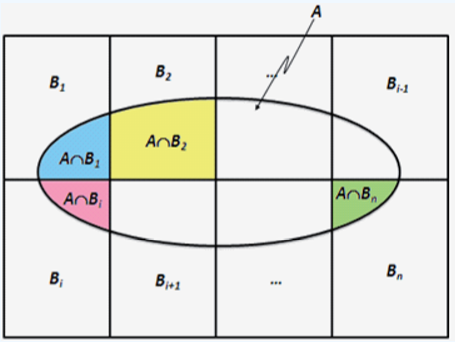
\includegraphics[scale=0.6]{pictures/image4.png}
    \centering
\end{figure}

\subsubsection{Teorema de Bayes}\label{eqn:bayes}

Considerem $A_1,\space A_2,\ldots,\space A_n$ una partició de $\Omega$. Llavors:
\begin{align*}
P(A_i\mid B) = \dfrac{P(B \mid A_i) \cdot P(A_i)}{\displaystyle\sum_{k=1}^{n} P(B\mid A_k)\cdot P(A_k)}
\end{align*}

Teorema deduible aplicant:
\begin{itemize}
    \item Probabilitat Total (\ref{eqn:ptotal})
    \item $P(A\cap B) = P(A) \cdot P(B\mid A)$ (\ref{eqn:condicionada})
    \item $P(A\cap B) = P(B\cap A)$ (\ref{eqn:condicionada})
\end{itemize}

\underline{Exemple 1:} Una malaltia afecta l’1\% de la població. Disposem d’un test que té una probabilitat
0.05 de donar un fals negatiu i 0.02 de donar un fals positiu. Es tria una persona a l’atzar i se li fa
el test. \\\\
(a) Quina és la probabilitat que el test doni positiu?\\
(b) Una persona triada a l’atzar d´ona positiu en el test.
Quina ´es la probabilitat que estigui malalta?

$(a)$ Probabilitat Total (\ref{eqn:ptotal})
\begin{itemize}
    \item $M=$ ``Persona malaltia'',\space\space $\overline{M}=$ ``Persona NO malaltia'', \quad $P(M) = 0.01$, \space $P(\overline{M}) = 0.99$
    \item $N=$ ``Test dona  negatiu'', \quad $P=$ ``Test dona  positiu''
    \item $N \mid M=$ ``Test dona negatiu i persona malaltia'', $P(N \mid M)=0.05$
    \item $P \mid \overline{M}=$ ``Test dona positiu i persona NO malaltia'', $P(P \mid \overline{M})=0.002$
\end{itemize}

$P(P) = P(P\mid M)\cdot P(M) +  P(P\mid \overline{M})\cdot P(\overline{M})$ \\\\
$P = \overline{N}, \quad P(\overline{N}\mid M) = 1-P(N\mid M)$ \\\\
$P(P)=\left[1-P(N\mid M)\right] \cdot P(M) + P(P\mid \overline{M})\cdot P(\overline{M}) = (1-0.05)\cdot 0.01 + 0.02\cdot 0.99 = 0.0293$

$(a)$ Teorema de Bayes (\ref{eqn:bayes})

$P(M\mid P) = \dfrac{P\cap M}{P(P)} =  \dfrac{P(M) \cdot P(P\mid M)}{P(P)} = \dfrac{0.01 \cdot (1-0.05)}{0.0293} = 0.324$ \\\\

\underline{Exemple 2:} Tenim 6 urnes $U_k$, $k = 1, \ldots , 6$ contenint $U_k$ $k$ boles blanques i $6-k$ boles negres.
Es tira un dau i s’extreu una bola a l’atzar de la urna corresponent al resultat del dau. Si la bola
és blanca, quina és la probabilitat que el dau hagués tret 3?
\begin{itemize}
    \item $U_k=$ ``treure la bola de la urna $k$, \quad $P(U_k) = \dfrac{k}{6}$
    \item $B=$ ``treue bola blanca'', \space $\overline{B}=$ ``treure bola negra''
    \item $B\mid U_k=$ ``treure bola blanca si la urna es k'', \quad $P(B\mid U_k) = \dfrac{k}{6}$
    \item $\overline{B}\mid U_k=$ ``treure bola negra si la urna es k'', \quad $P(\overline{B}\mid U_k) = 1 - P(B\mid U_k) = 1 - \dfrac{k}{6}$
\end{itemize}

Ens estan preguntant $\rightarrow P(U_3\mid B)$

Ho podem resoldre directament aplicant el Teorema de Bayes (\ref{eqn:bayes}) i Serie Aritmètica (\ref{eqn:saritmetica}):
\begin{align*}
P(U_3\mid B) = \dfrac{P(B\mid U_3) \cdot P(U_3)}{\displaystyle\sum_{k=1}^{6} P(B\mid U_k)\cdot  P(U_k)} = \dfrac{\dfrac{3}{6} \cdot \dfrac{1}{6}}{\dfrac{1}{36} \cdot \displaystyle\sum_{k=1}^{6} k} = \dfrac{3}{\dfrac{6 \cdot 7}{2}} = \dfrac{1}{7} = 0.143
\end{align*}

\newpage
\section{Variables Aleatòries}

\subsection{Definició}

Una variable aleatòria és un valor numéric que correspon a un resultat d'un experiment aleatòri, del qual no sabem amb certesa el seu resultat, però si el podem modelitzar mitjançant les variables aleatòries. Exemples: 

\begin{itemize}
    \item $X=$ Número de cares obtingudes al llençar una moneda $n$ vegades \\
    $P(X=2),$ $P(X=3),$ $\ldots$
    \item $X=$ Número de vegades que ha sortit 6 llençant un dau $n$ vegades \\
    $P(X=1),$ $P(X=2),$ $\ldots$
    \item $X=$ Possibles resultats llençant un dau 2 vegades \\
    $P(X=\textrm{``senar''}),$ $P(X=\textrm{``sumin 7''})$, $P(X=\textrm{``cap 2''}),$ $\ldots$
    \item $X=$ Temperatura màxima mesurada en un día en una ciutat concreta \\
    $P(X=37),$ $P(X\geq20),$ $\ldots$
    \item $X=$ Número de trucades que rep una linea telefónica durant un temps determinat $t$\\
    $P(X=10),$ $P(X\geq10),$ $\ldots$
\end{itemize}

Per un experiment donat hi ha infinitat de variables aleatòries. Les variables aleatòries són els objectes que utilitzem quan fem un tractament probabilístic d’una situació real i ens ajuden a modelitzar i a estimar aquests processos reals d'una forma probabilística.

\subsection{Funció de Distribució Acumulada (FDA)}

Donada una variable aleatòria $X$, definim la seva Funció de Distribució Acumulada (FDA) o a vegades anomenada simplemente Funció de Distribució (FD) com:
\begin{align*}
F_X(x) = P(X\leq x)
\end{align*}

És, per tant, la probabilitat de l’interval $(-\infty, x]$. Si coneixem la funció $F_X$, queden determinades totes les probabilitats de la variable aleatòria, doncs la FDA evaluada en un número $x$ qualsevol és la probabilitat de que la variable aleatoria prengui un valor menor o igual a $x$.

Immediatament trobem que donats $a \leq b \rightarrow P(a < X \leq b) = F_X(b) - F_X(a)$.

Propietats:

\begin{itemize}
    \item $0 \leq F_X(x) \leq 1$
    \item $F_X$ es una funció sempre creixent
\end{itemize}


\subsection{Funció de Densitat de Probabilitat (FDP)}

Donada una variable aleatòria $X$, definim la funció de Densitat de Probabilitat (FDP) o simplemente Funció de Densitat ($f_X$ continua, $P_X$ discreta) com la funció que descriu la probabilitat relativa, segons la qual la cual aquesta variable aleatòria pendrá un determinat valor. Un histograma de probabilitat.

Propietats VA continua:
\begin{itemize}
    \item $f_X \geq 0$
    \item $P(X=x_1) = f_X(x_1)$
    \item $P(a \leq x \leq b) = \displaystyle \int_{a}^{b} f_X(x) \cdot dx$
    \item $F_X(x) = \displaystyle \int_{-\infty}^{b} f_X(x') \cdot dx'$
    \item $f_X = \dfrac{dF_X(x)}{dx}$
\end{itemize}

Propietats VA Discreta:

\begin{itemize}
    \item $P_X \geq 0$
    \item $P(X=k) = P_X(k) = F_X(k) - F_X(k-1) \rightarrow$ Ho podem verue en la figura (\ref{fig:fda})
    \item $P(a \leq X \leq b) = \displaystyle \sum_{k=a}^{b} P_X(k)$
    \item $F_X(k) = \displaystyle \sum_{i=-\infty}^{k} P_X(i)$
\end{itemize}

\subsection{Variables aleatòries discretes}
Una variable aleatòria discreta es la que pren un valor finit de valors. Si aquests valors són ordenats: $x_1, x_2, \ldots, x_n$
amb probabilitats $p_1, p_2, \ldots , p_n$, $F_X$ és una funció esglaonada que pren valors $0, p_1, p_1 + p_2, \ldots , p_1+ \ldots + p_{n-1}, 1$. Tota $F_X$ per una variable aleatoria discreta es pot calcular utilitzant la funció de Heaviside $u(x)$ (\ref{heaviside}).

\begin{align*}
F_X(k) = \displaystyle \sum_{k} P(k=i) \cdot u(k-i)
\end{align*}
\begin{align*}
P_X(k) = F_X(k) - F_X(k-1)
\end{align*}
\begin{figure}[H]
    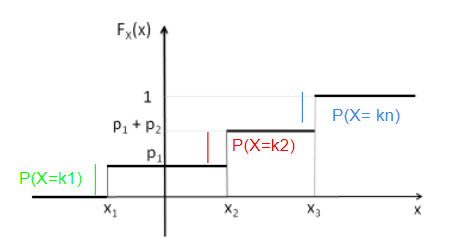
\includegraphics[scale=0.7]{pictures/image7.png}
    \centering
    \caption{Funció de distribució d’una variable discreta.}
    \label{fig:fda}
\end{figure}

A continuació veurem les VA's discretes més importants.

\subsubsection{Bernoulli}
Essent $X$ una VA, es considera de Bernoulli quan mesura el resultat d'un \textbf{experiment aleatòri amb tan sols 2 resultats possibles}, denominats exit i fracàs. 
\begin{itemize}
    \item $P(\textrm{``éxit''}) = p$
    \item $P(\textrm{``no éxit''}) = P(\textrm{``fracas''}) = q = 1-p$ 
\end{itemize}
\begin{align*}
    X \sim B(p)
\end{align*}

\subsubsection{Binomial}
Essent $X$ una VA, es considera Binomial quan modelitza \textbf{exactament} el \textbf{nombre d'éxits $(k)$} en una seqüencia d'$n$ \textbf{experiments de Bernoulli independents} entre si, amb una probabilitat d'èxit fixa $p$ i una probabilitat de fracàs fixa $q$. 
\begin{align*}
    X \sim BN(n,p)
\end{align*}

\begin{itemize}
    \item $n:$ nombre d'experiments de Bernoulli
    \item $p:$ probabilitat d'èxit
    \item $q = 1 - p:$ probabilitat de fracàs
\end{itemize}
\begin{align*}
    P_X(k) = P(X=k) = \dbinom{n}{k} \cdot p^k \cdot (1-p)^{n-k}
\end{align*}

\textbf{DEM:} Suposem el llançament d'una dau no trucat com experiment de Bernoulli a repetir $n$ vegades i VA $X$ el nombre de tresos.
\begin{itemize}
    \item p = $\dfrac{1}{6}$
    \item q = $\dfrac{5}{6}$
\end{itemize}
$P(X=k)$ es la probabilitat que hi hagi $k$ tresos en una seqüencia de $n$ elements, per tan, $k$ tresos i $n-k$ qualsevol altre numero. Com son independents, la probabilitat d'una seqüencia com aquesta és $p^k \cdot q^{n-k}$, ja que per independència anem multiplicant la probabilitat de cada resultat individual.

Ara falt afegir el combinatori $\dbinom{n}{k}$, que equival al numero de maneres posibles en les que podem ordenar aquesta seqüencia, es a dir, situar els $k$ tresos entre la resta de resultats.

\begin{blocktemplate}{NOTA}
La \textbf{distribució binomial} s'utiliza amb freqüencia per a modelizar exactament el número d'èxits en una mostra de $k$ elements extreta amb \textbf{remplaçament} d'una población d' $n$. Si les extraccions es realitzen \textbf{sense replaçament no son independients}, per tant la VA resultant no es una distribució binomial, si no una hipergeomètrica (\ref{hipergeom}. Tot i això, si $n >> k$ la distribució binomial segueix essent una bona aproximació, i s'utilitza ampliament.
\end{blocktemplate}

\begin{blocktemplateI}{NOTA 2}
Si en comptes del número d'èxits $k$, volem calcular $k$ o més èxits, haurem de sumar les probabilitats individuals de cadascuna d'aquestes $k$. No es necessari extreure la intersecció, doncs si ho pensem en deteniment, de seguida ens adonarem que existeix la intersecció entre `A' i `B', doncs no pots tenir alhora tant \textbf{exactament} 27 èxits com exactament 28 èxitos en 30 assajos. Pots tener \textbf{exactament} 27 o \textbf{exactament} 28 perà mai els dos a l'hora (intersecció).
\end{blocktemplateI}

\paragraph{Algunes Propietats}

\paragraph{FDA i FDP}

\paragraph{Paràmetres Estadístics}

\paragraph{Exemples}

\subsubsection{Hipergeomètrica} \label{hipergeom}
Essent $X$ una VA, es considera Hipergeomètrica quan modelitza el \textbf{nombre d'éxits $(k)$} en una seqüencia d'$n$ \textbf{experiments de Bernoulli DEPENDENTS} entre si, amb una probabilitat d'èxit fixa $p$ i una probabilitat de fracàs fixa $q$. 

\begin{itemize}
    \item $n:$ nombre d'experiments de Bernoulli
    \item $N:$ població total d'elements
    \item $K:$ elements que pertanyen a la categoria A
    \item $N-K:$ elements que pertanyen a la categoria B
\end{itemize}
\begin{align*}
    X \sim HG(N,K,n), \quad P(X=k) = \dfrac{\dbinom{K}{k} \cdot \dbinom{N-K}{n-k}}{\dbinom{N}{n}}
\end{align*}

\textbf{NOTA:} El cas d'us típic de la VA Hipergeomètrica es quan tenim una població d'$n$ elements, dels quals:

\begin{itemize}
    \item $k$ pertanyen a la categoria $A$
    \item $n-k$ pertanyen a la categoria $A$
\end{itemize}

La distribució hipergeomètrica modelitza la probabilitat d'obtindre \textbf{exactament} $k$ elements de la categoría $A$ amb extraccions sense remplaçament.

\paragraph{FDA i FDP}

\paragraph{Paràmetres Estadístics}

\paragraph{Exemples}
POKER FULL


\subsubsection{Geomètrica}
Essent $X$ una VA, es considera Geomètrica quan modelitza el \textbf{nombre total d'intents} fins obtindre el primer \textbf{èxit} ($k$) en una successió d'\textbf{esdeveniments} \textbf{independents} de \textbf{Bernoulli}, essent $p$ la probabilitat d'èxit.

\begin{align*}
    X \sim Geo(p), \quad P(X=k) = p \cdot (1-p)^{k-1}
\end{align*}

\paragraph{FDA i FDP}

\paragraph{Paràmetres Estadístics}

\paragraph{Exemples}

\subsubsection{Poisson}


\subsection{FDA y FDP Condicionadas}
\begin{align*}
F_X(x \mid B) = P(X\leq x\mid B) = \dfrac{P(X\leq x\cap B)}{P(B)}
\end{align*}

VA Continua:
\begin{itemize}
    \item $f_X(x \mid B) = \dfrac{dF_X(x\mid B)}{dx}$
    \item Aplicant Teorema de Bayes (\ref{eqn:bayes}) $\rightarrow f(x\mid B) = \dfrac{P(B\mid X=x)\cdot f_X(x)}{\displaystyle \int_{-\infty}^{\infty} P(B\mid X=x')\cdot f_X(x') \cdot dx'}$
\end{itemize}

VA Discreta:
\begin{itemize}
    \item Aplicat P.Total (\ref{eqn:ptotal}) $\rightarrow P_X(k) = \displaystyle \sum_{i=1}^{n}P_{X}(k|Ai)\cdot P(Ai)$
    \item Aplicant Teorema de Bayes (\ref{eqn:bayes}) $\rightarrow P_{X}(k\mid B) = \dfrac{P(B\mid X=k)\cdot P_X(k)}{\displaystyle \sum_{i=-\infty}^{\infty} P(B\mid i)\cdot P_X(i)}$
\end{itemize}

\subsection{Variables aleatòries discretes comuns}

\subsection{Variables aleatòries continues comuns}

\newpage
\section{Paràmetres Estadístics}

\newpage
\section{Apèndix}

\subsection{Series}

\subsubsection{Serie Aritmètica}\label{eqn:saritmetica}

\begin{align*} 
\sum_{i=1}^{n} a_i = \dfrac{n \cdot (a_1 + a_n)}{2}
\end{align*}

\subsubsection{Serie Geomètrica} \label{eqn:sgeometrica}

\begin{align*}
&S_{n+1} = 1 + r + r^2 + r^3 + \ldots + r^n =  \sum_{i=0}^{n} r^{i} = \dfrac{1-r^{n+1}}{1-r} \\
&S_{n} = r + r^2 + r^3 + \ldots + r^n =  S_{n+1} - 1 = \sum_{i=1}^{n} r^{i} = \dfrac{r-r^{n+1}}{1-r}
\end{align*}

\subsection{Funcions}

\subsubsection{Heaviside} \label{heaviside}
\begin{align*}
u(t) =
\left\{
	\begin{array}{ll}
		0  & \mbox{if } t < 0 \\
		  1 & \mbox{if } t \geq 0
	\end{array}
\right.
\end{align*}
\begin{figure}[H]
    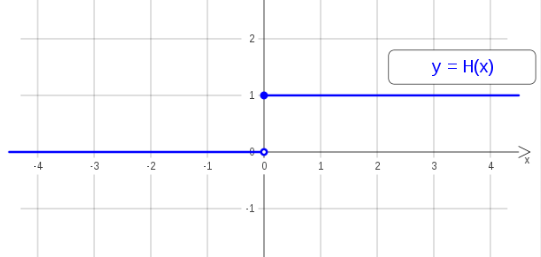
\includegraphics[scale=0.6]{pictures/image6.png}
    \centering
\end{figure}
\begin{align*}
u(t-a) =
\left\{
	\begin{array}{ll}
		0  & \mbox{if } t < a \\
		  1 & \mbox{if } t \geq a
	\end{array}
\right.
\end{align*}

\begin{figure}[H]
    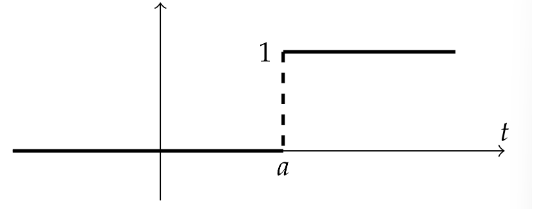
\includegraphics[scale=0.6]{pictures/image5.png}
    \centering
\end{figure}
\end{document}
